\section{The performance of Split-DASH Architecture}
Before we can start playing with Split-DASH
\begin{figure}[ht]
	\captionsetup[subfigure]{}
	\begin{center}
		\subfloat[\label{fig:avgQl}Average Bit-rate]{
			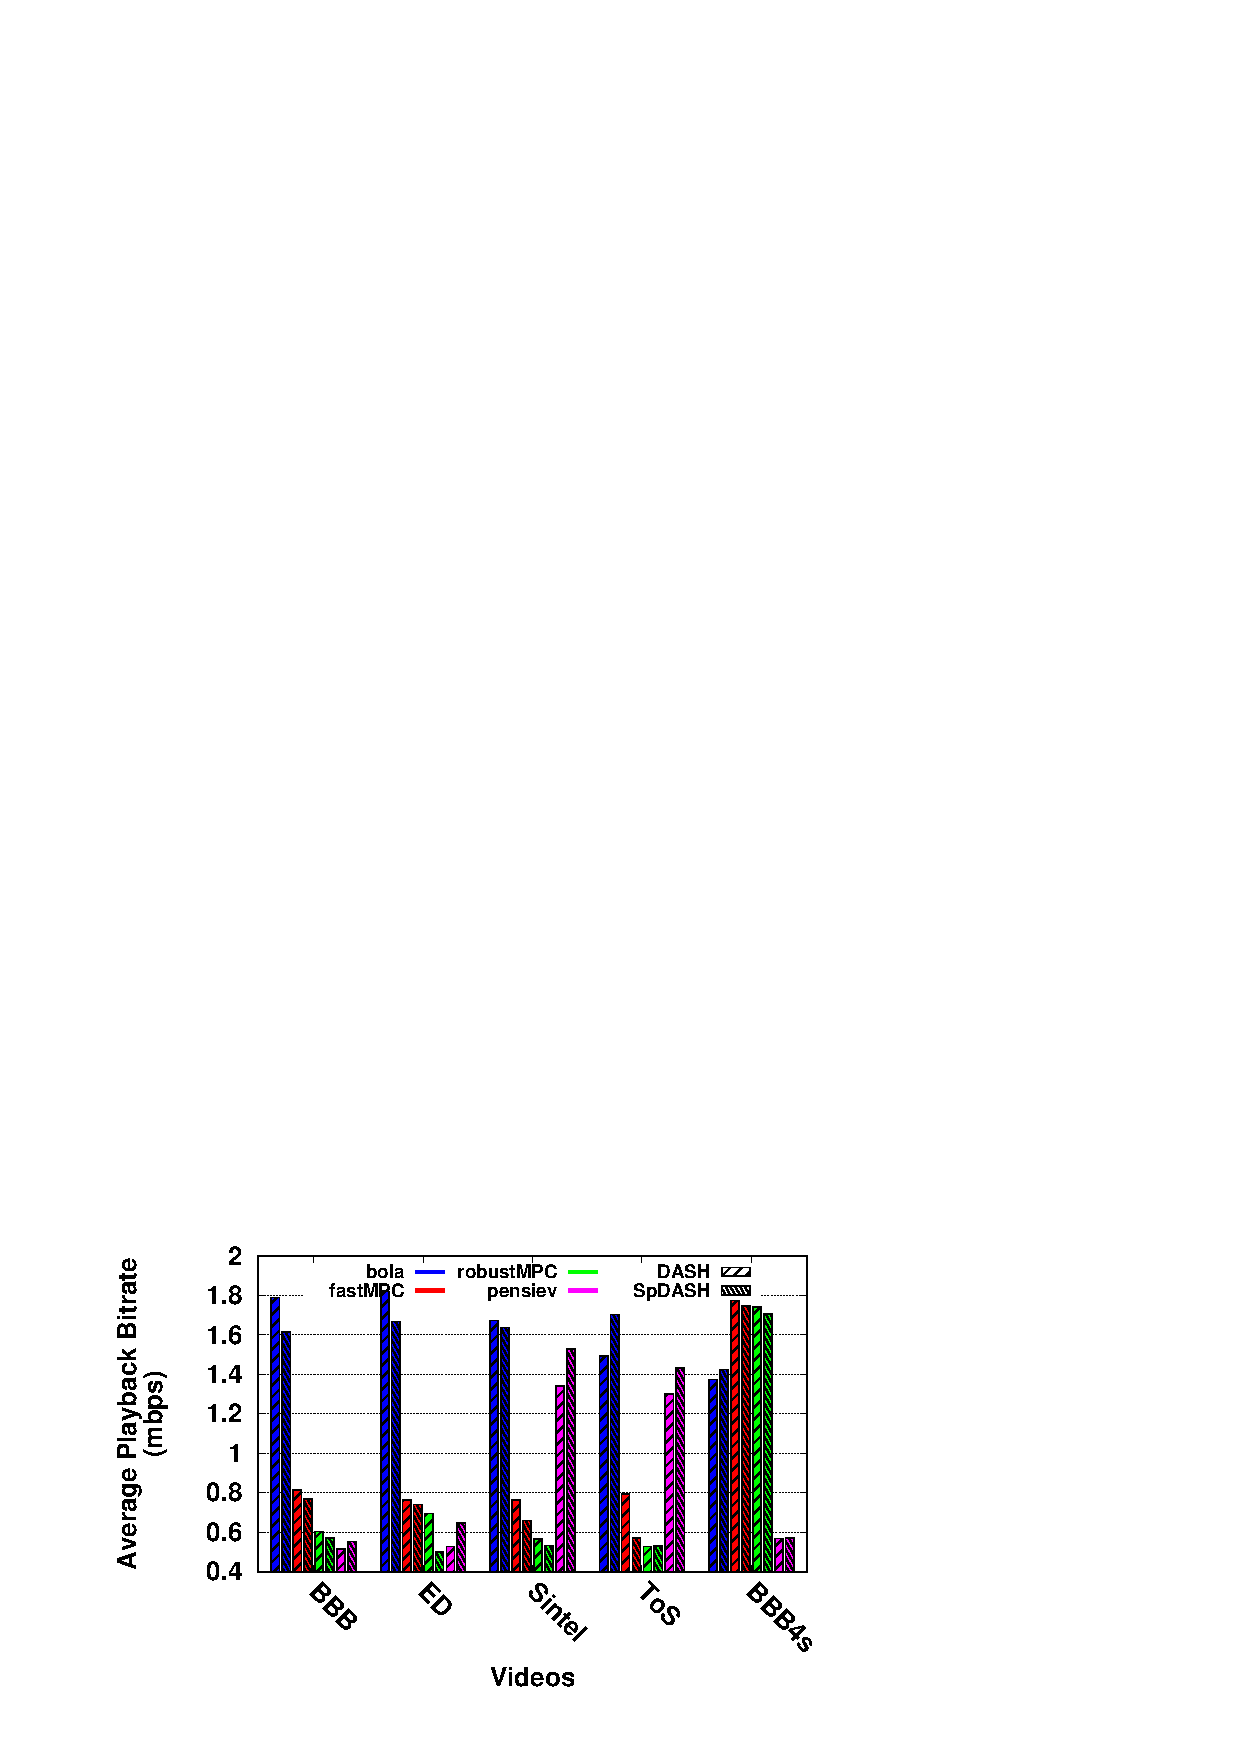
\includegraphics[width=0.49\linewidth]{img/spdash/avgQl}
		}
		\subfloat[\label{fig:avgQlVar}Bit-rate Variation]{
			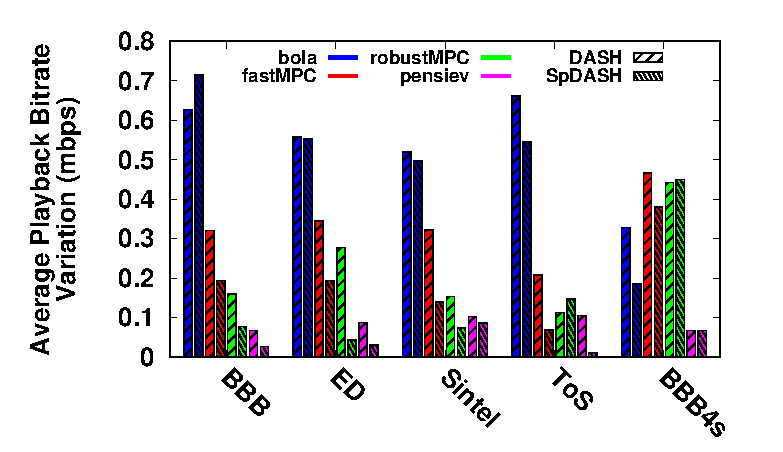
\includegraphics[width=0.49\linewidth]{img/spdash/avgQlVar}
		}
	
		\subfloat[\label{fig:avgStall}Bit-rate Variation]{
			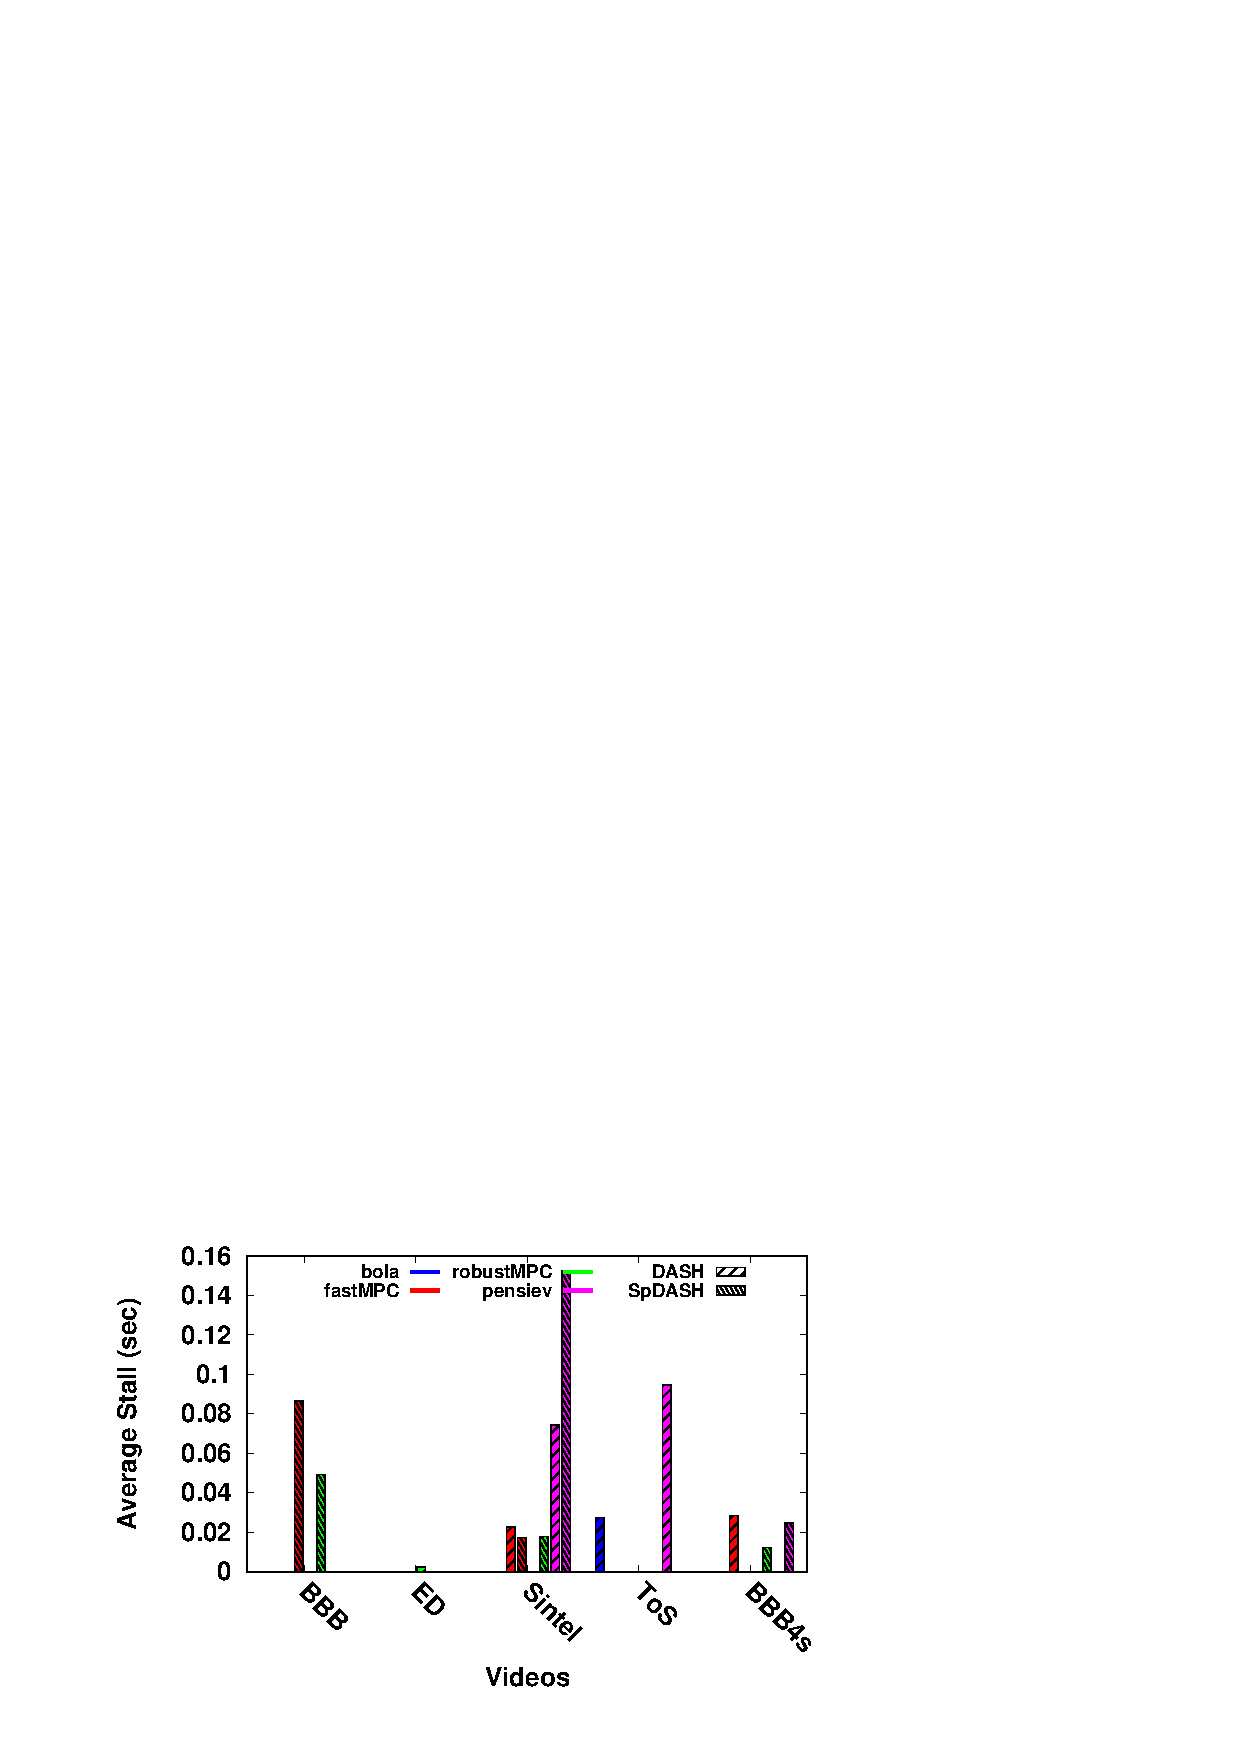
\includegraphics[width=0.49\linewidth]{img/spdash/avgStall}
		}
		\subfloat[\label{fig:qoe}Bit-rate Variation]{
			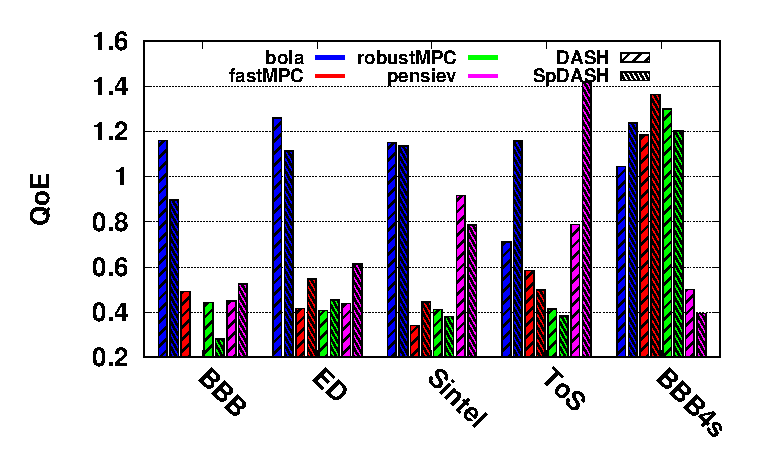
\includegraphics[width=0.49\linewidth]{img/spdash/qoe}
		}
	\end{center}
	\caption{\label{fig:avgBitrate} QoE Components: Average Bit-rate and Bit-rate Variation}
\end{figure}

%\begin{figure*}
%	\centering
%	\begin{subfigure}{.23\linewidth}
%		\centering
%		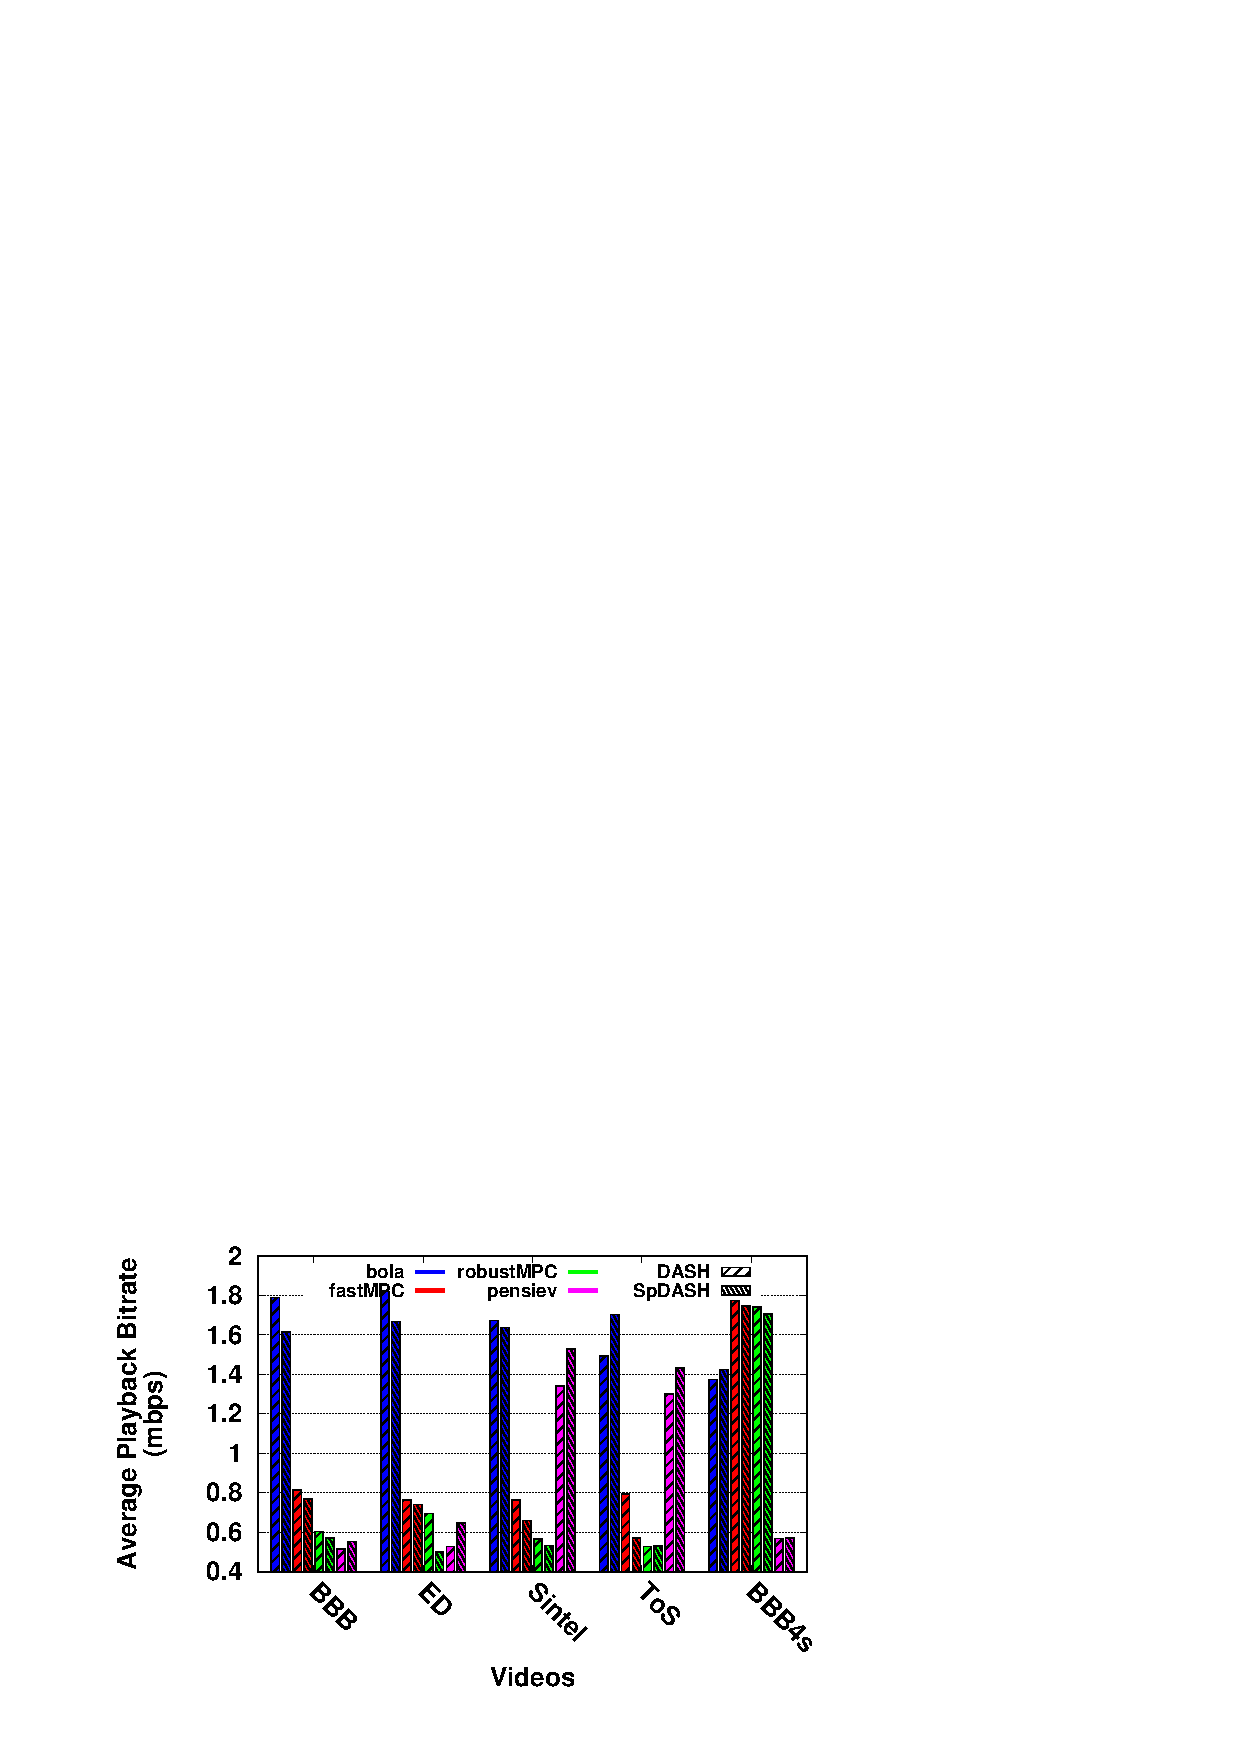
\includegraphics[width=1\linewidth]{img/spdash/avgQl}
%		\caption{BOLA}
%	\end{subfigure}
%	\begin{subfigure}{.23\linewidth}
%		\centering
%		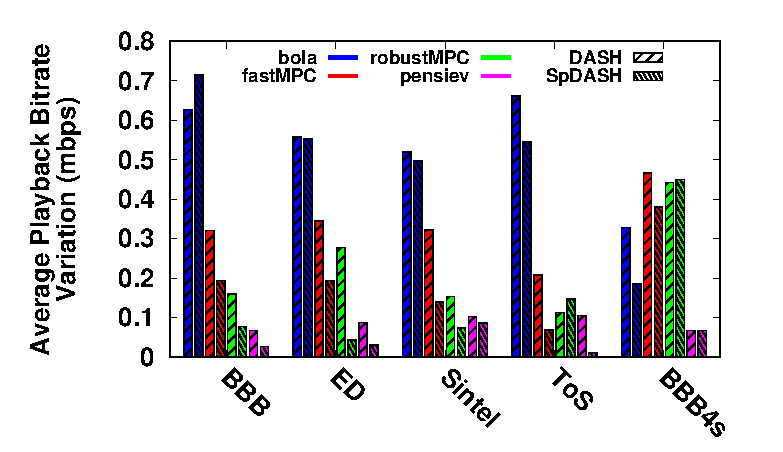
\includegraphics[width=1\linewidth]{img/spdash/avgQlVar}
%		\caption{MPC-fast}
%	\end{subfigure}
%	\begin{subfigure}{.23\linewidth}
%		\centering
%		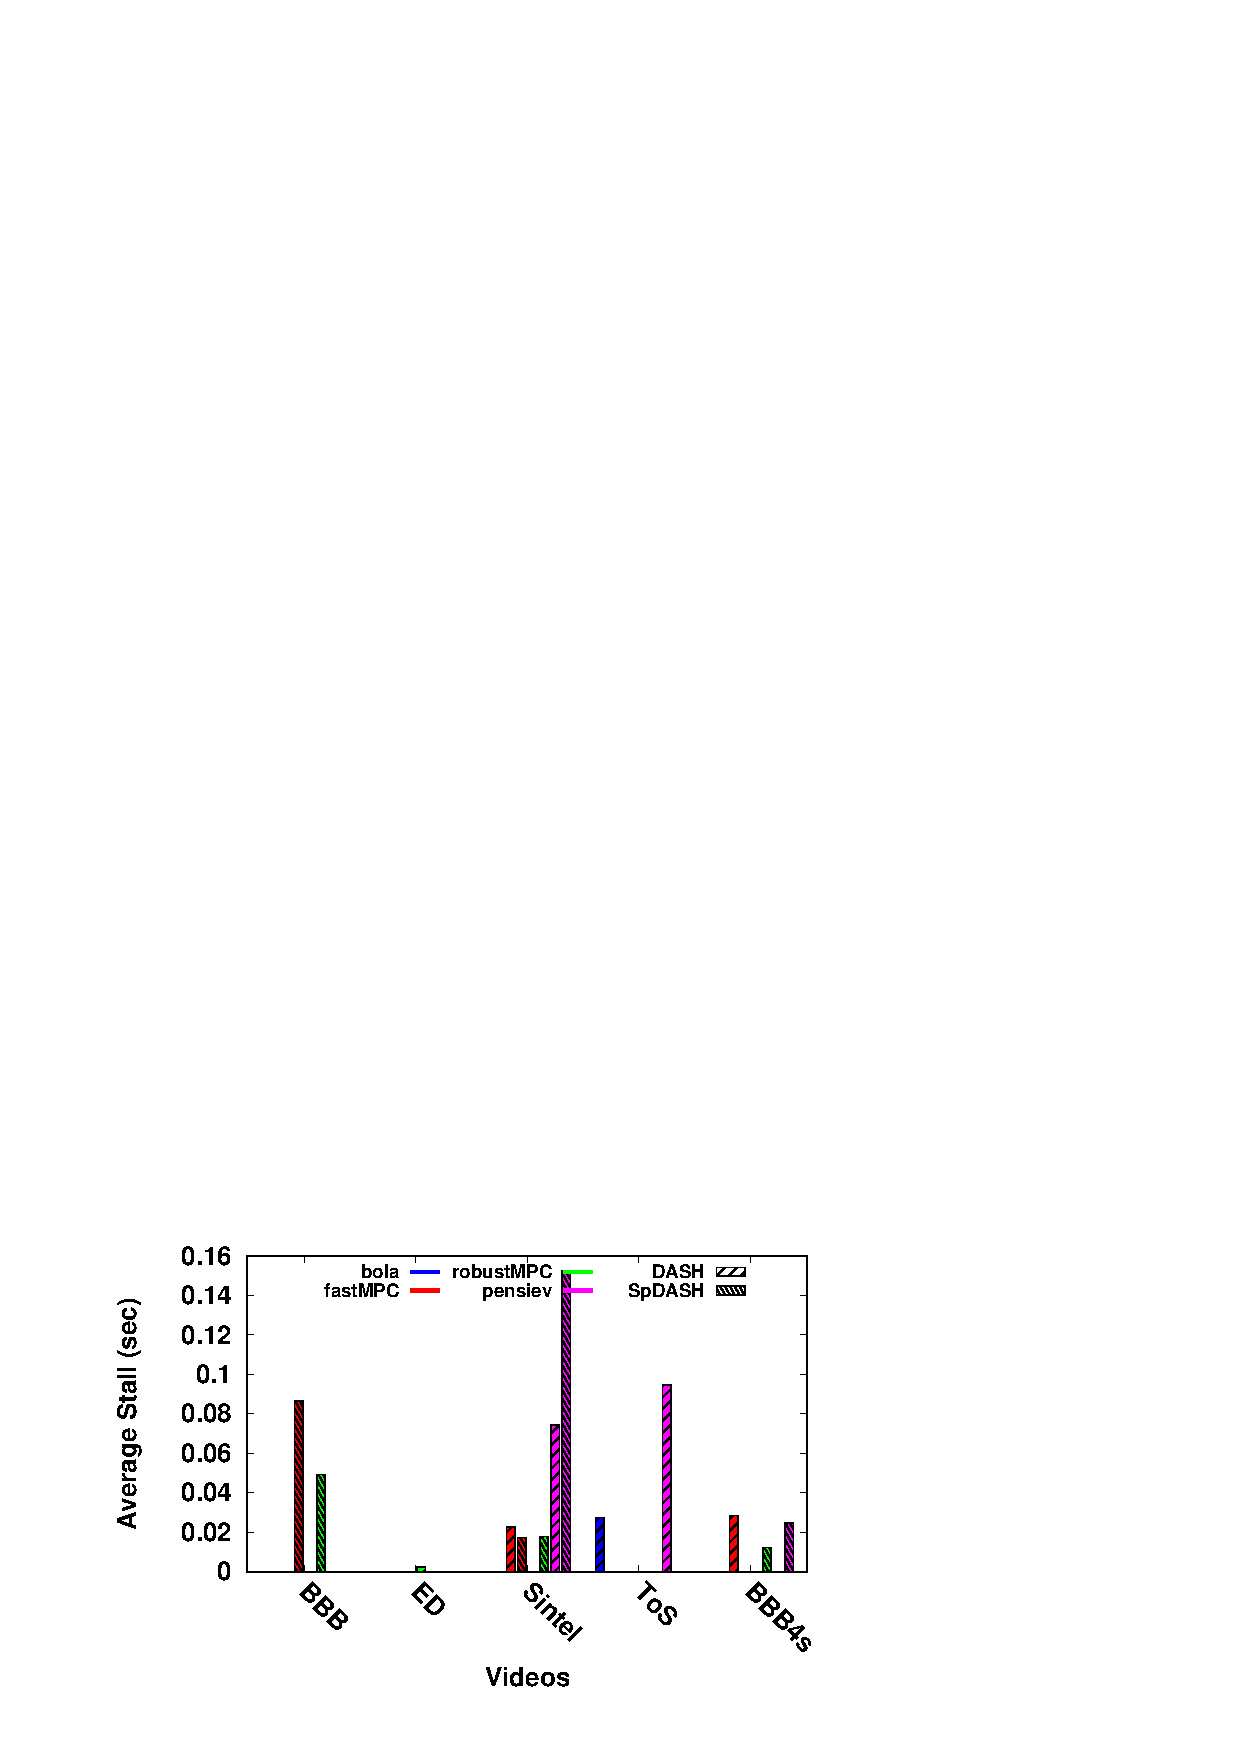
\includegraphics[width=1\linewidth]{img/spdash/avgStall}
%		\caption{MPC-robust}
%	\end{subfigure}
%	\begin{subfigure}{.23\linewidth}
%		\centering
%		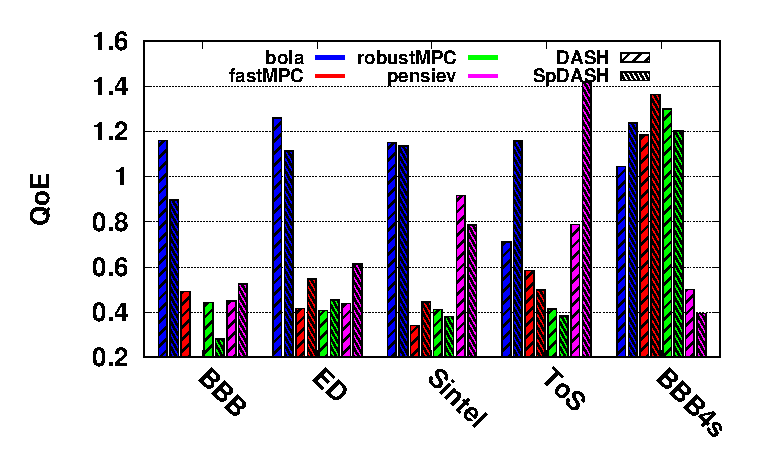
\includegraphics[width=1\linewidth]{img/spdash/qoe}
%		\caption{MPC-robust}
%	\end{subfigure}
%	\caption{\label{fig:fairness_bitrate}Average playback bitrate while players share common bottleneck but starts in separate times.}
%\end{figure*}